%!TEX root=Principal.tex
\chapter{PROPOSTA}
\label{cap:proposta}

Este trabalho apresenta uma metodologia que mapeia o conjunto de ações que o robô é capaz de executar visando a maximização a qualidade da interação humano-robô, baseando-se no comportamento e características do indivíduo. Como observado ao longo dos trabalhos da literatura apresentados até agora, o comportamento do indivíduo possui dependência da origem ou cultura dele. Assim, algumas reações apresentadas por uma pessoa podem ser influenciadas pelo local de nascimento, pelos locais que o indivíduo viveu e também pela sua experiência de vida. Contudo, fatores como a experiência de vida e cultura são difíceis de avaliar apenas com a observação de uma determina pessoa.

Dessa forma, a técnica de Raciocínio baseado em Casos (RBC) foi escolhida como apoio a essa tese, para que seja possível armazenar as experiências de interações entre robô e as pessoas, e a partir da informação gerada com base nos casos, identificar a melhor forma de interagir com novas pessoas de acordo com seu perfil comportamental. Entretanto, o número de informação gerada no processo de interação com diversas pessoas é consideravelmente alto, isso dificulta a consulta dos casos para reutilizar a solução em tempo de interação entre o ser humano e o robô. Com o intuito de minimizar a quantidade de casos para encontrar a provável melhor interação tendo como base um determinado perfil e otimizar o tempo de procura dessa solução é utilizado um algoritmo de agrupamento que será capaz de gerar grupos de perfis comportamentais. É a partir desses perfis que o mecanismo de classificação identifica o melhor conjunto de ações para o robô executar referente àquele caso. 

Essa seção apresenta em detalhes os passos da metodologia proposta por esta tese. Ao final do capítulo é apresentado a visão completa da metodologia onde é realizado uma síntese do processo como um todo e das técnicas aplicadas nele. Antes de entrar em detalhes na metodologia, é apresentado o robô que será utilizado para o desenvolvimento do estudo proposto nessa tese.

\section{O Robô}
\label{sec:robo}
O robô utilizado no desenvolvimento dessa tese é o PeopleBot~\footnote{PeopleBot - http://www.mobilerobots.com/researchRobots/PeopleBot.aspx} fabricado pela ActivMedia Robotics. Ele é um robô móvel com direção diferencial, ou seja, possui duas rodas motorizadas e uma roda castor que auxilia no equilíbrio do robô. O projeto do PeopleBot tem foco em pesquisas e serviços que envolvem interação humano-robô, devido a isso ele possui uma altura de 112 cm (centímetros). Além disso, o PeopleBot também possui uma garra pequena que tem sua movimentação apenas na vertical. A figura~\ref{fig:peoplebot} apresenta o robô PeopleBot.

\begin{figure}[ht!]
	\centering
	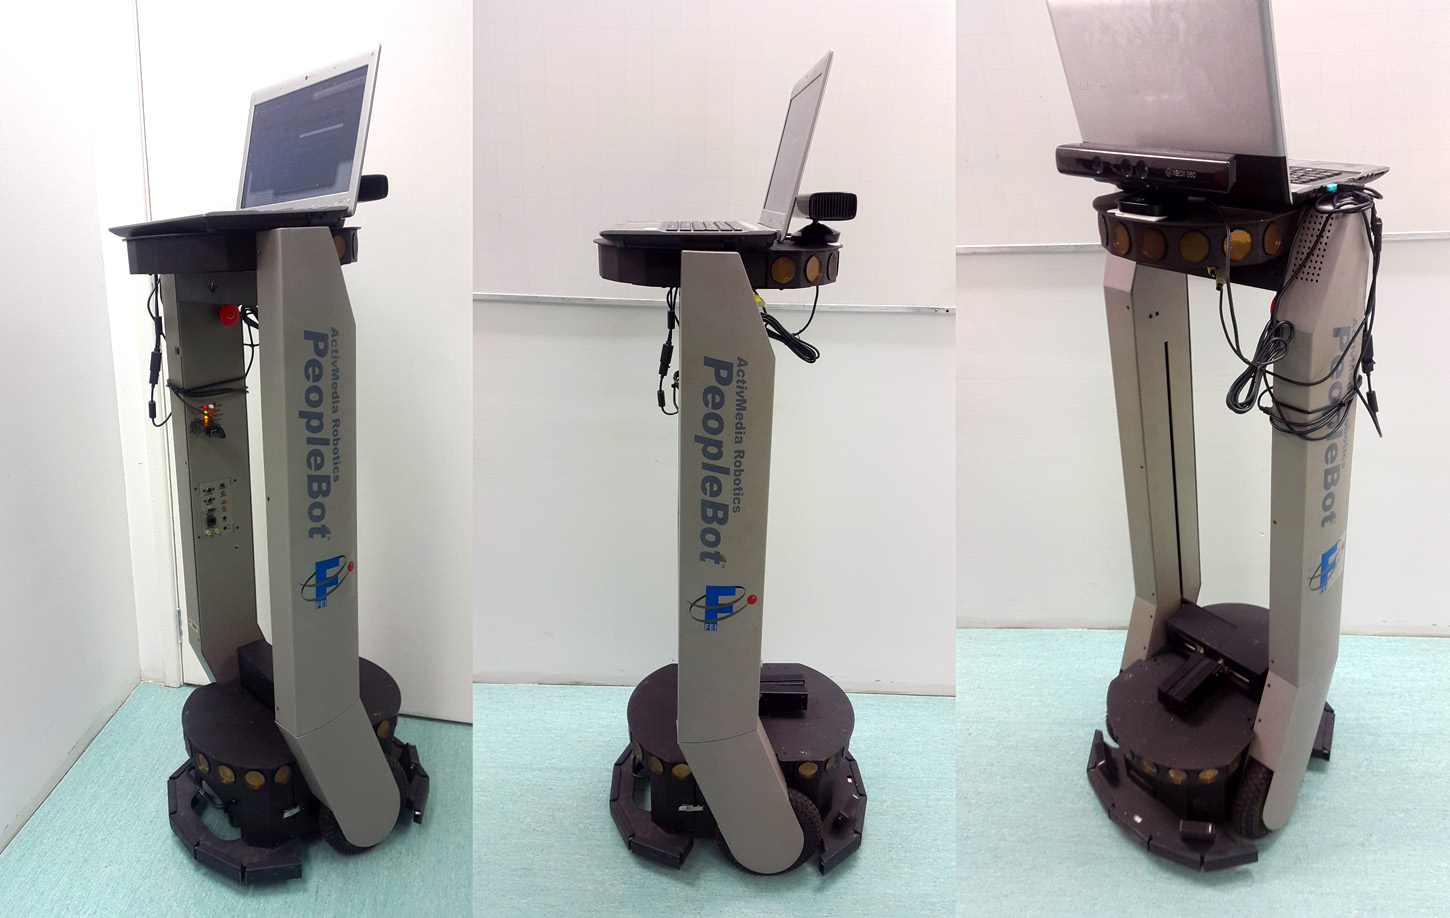
\includegraphics[width=\textwidth]{images/peoplebot.jpg}
	\caption{Robô ActivMedia Robotics PeopleBot.}
	\label{fig:peoplebot}
\end{figure}

Como a garra do PeopleBot é curta e não permite muitos movimentos, foi adicionado um manipulador para auxiliar na manipulação de objetos durante a interação com as pessoas e também na prestação de serviços domésticos e de cuidados pessoais. O projeto de construção do manipulador é apresentado através da figura~\ref{fig:manipulador}.

\begin{figure}[ht!]
	\centering
	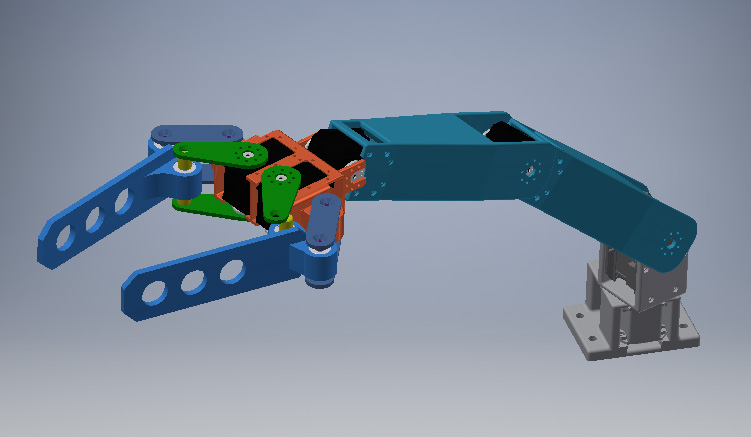
\includegraphics[width=0.6\textwidth]{images/manipulador.jpg}
	\caption{Projeto do Novo Manipulador do PeopleBot.}
	\label{fig:manipulador}
\end{figure}

O novo manipulador foi construído de maneira que os movimentos sejam parecidos com o braço humano. Além do manipulador, também será acoplado um \emph{tablet} para que seja possível atribuir faces ao robôs e deixar a interação mais amigável. Alguns sensores como o Microsoft\textregistered\ Kinect\textregistered\ e o ASUS\textregistered\ Xtion\textregistered\ também foram instalados para melhorar a captura das informações que são apresentadas na seção~\ref{sec:extracaocaracteristicas}, a seguir.

\section{Extração das Características para o RBC}
\label{sec:extracaocaracteristicas}

Como apresentado na seção \ref{cap:ihr}, existem diversas variáveis que podem auxiliar na extração de um perfil comportamental do individuo. \emph{Proxemics} tornam possível a extração de fatores sobre a distância social entre o individuo e o robô. Esses fatores podem variar não só entre a posição física dos dois agentes, mas também na posição do corpo dos indivíduos, como por exemplo, a orientação dos ombros e troco em relação a posição do robô. Outro fator também significante é a fixação entre olhares, este pode determinar o início e o fim de uma interação, além dos principais indivíduos na interação. Além disso, pode ser também empregado o reconhecimento de expressões faciais que auxiliam na análise do quanto a situação é confortável para o individuo, ou seja, o quanto ele está apreciando a interação, de tal forma, que possa existir uma avaliação em tempo real das reações deste durante todo o processo de interação. Outra técnica que pode ser utilizada na análise do conforto do individuo durante a interação é a avaliação da emoção através da voz da pessoa.

Dessa forma, é possível empregar diversos sensores que auxiliam a leitura e quantificação dessas variáveis. Sensores de captura de marcações de movimento, como Microsoft\textregistered\ Kinect\textregistered\ ou o ASUS\textregistered\ Xtion\textregistered, são utilizados para quantificar os valores obtidos através da \emph{Proxemic}, que envolvem distância entre agentes e orientação de membros do individuo. Para realizar o reconhecimento de expressões faciais utiliza-se uma câmera de video, podendo assim executar uma leitura da face do individuo em tempo de execução na interação entre o humano e o robô. As variáveis referentes a questão da fixação dos olhares dos agentes para identificar o início e o fim da interação, podem ser obtidas através de ambos sensores de tal forma, que seja possível determinar a orientação da cabeça e torso do individuo e também a direção do olhar deste para com o robô. A voz do individuo para análise da emoção na interação é obtida através de um microfone. A figura \ref{fig:capturacaracteristicas} apresenta a ilustração do processo de extração das características do individuo.

\begin{figure}[ht!]
	\centering
	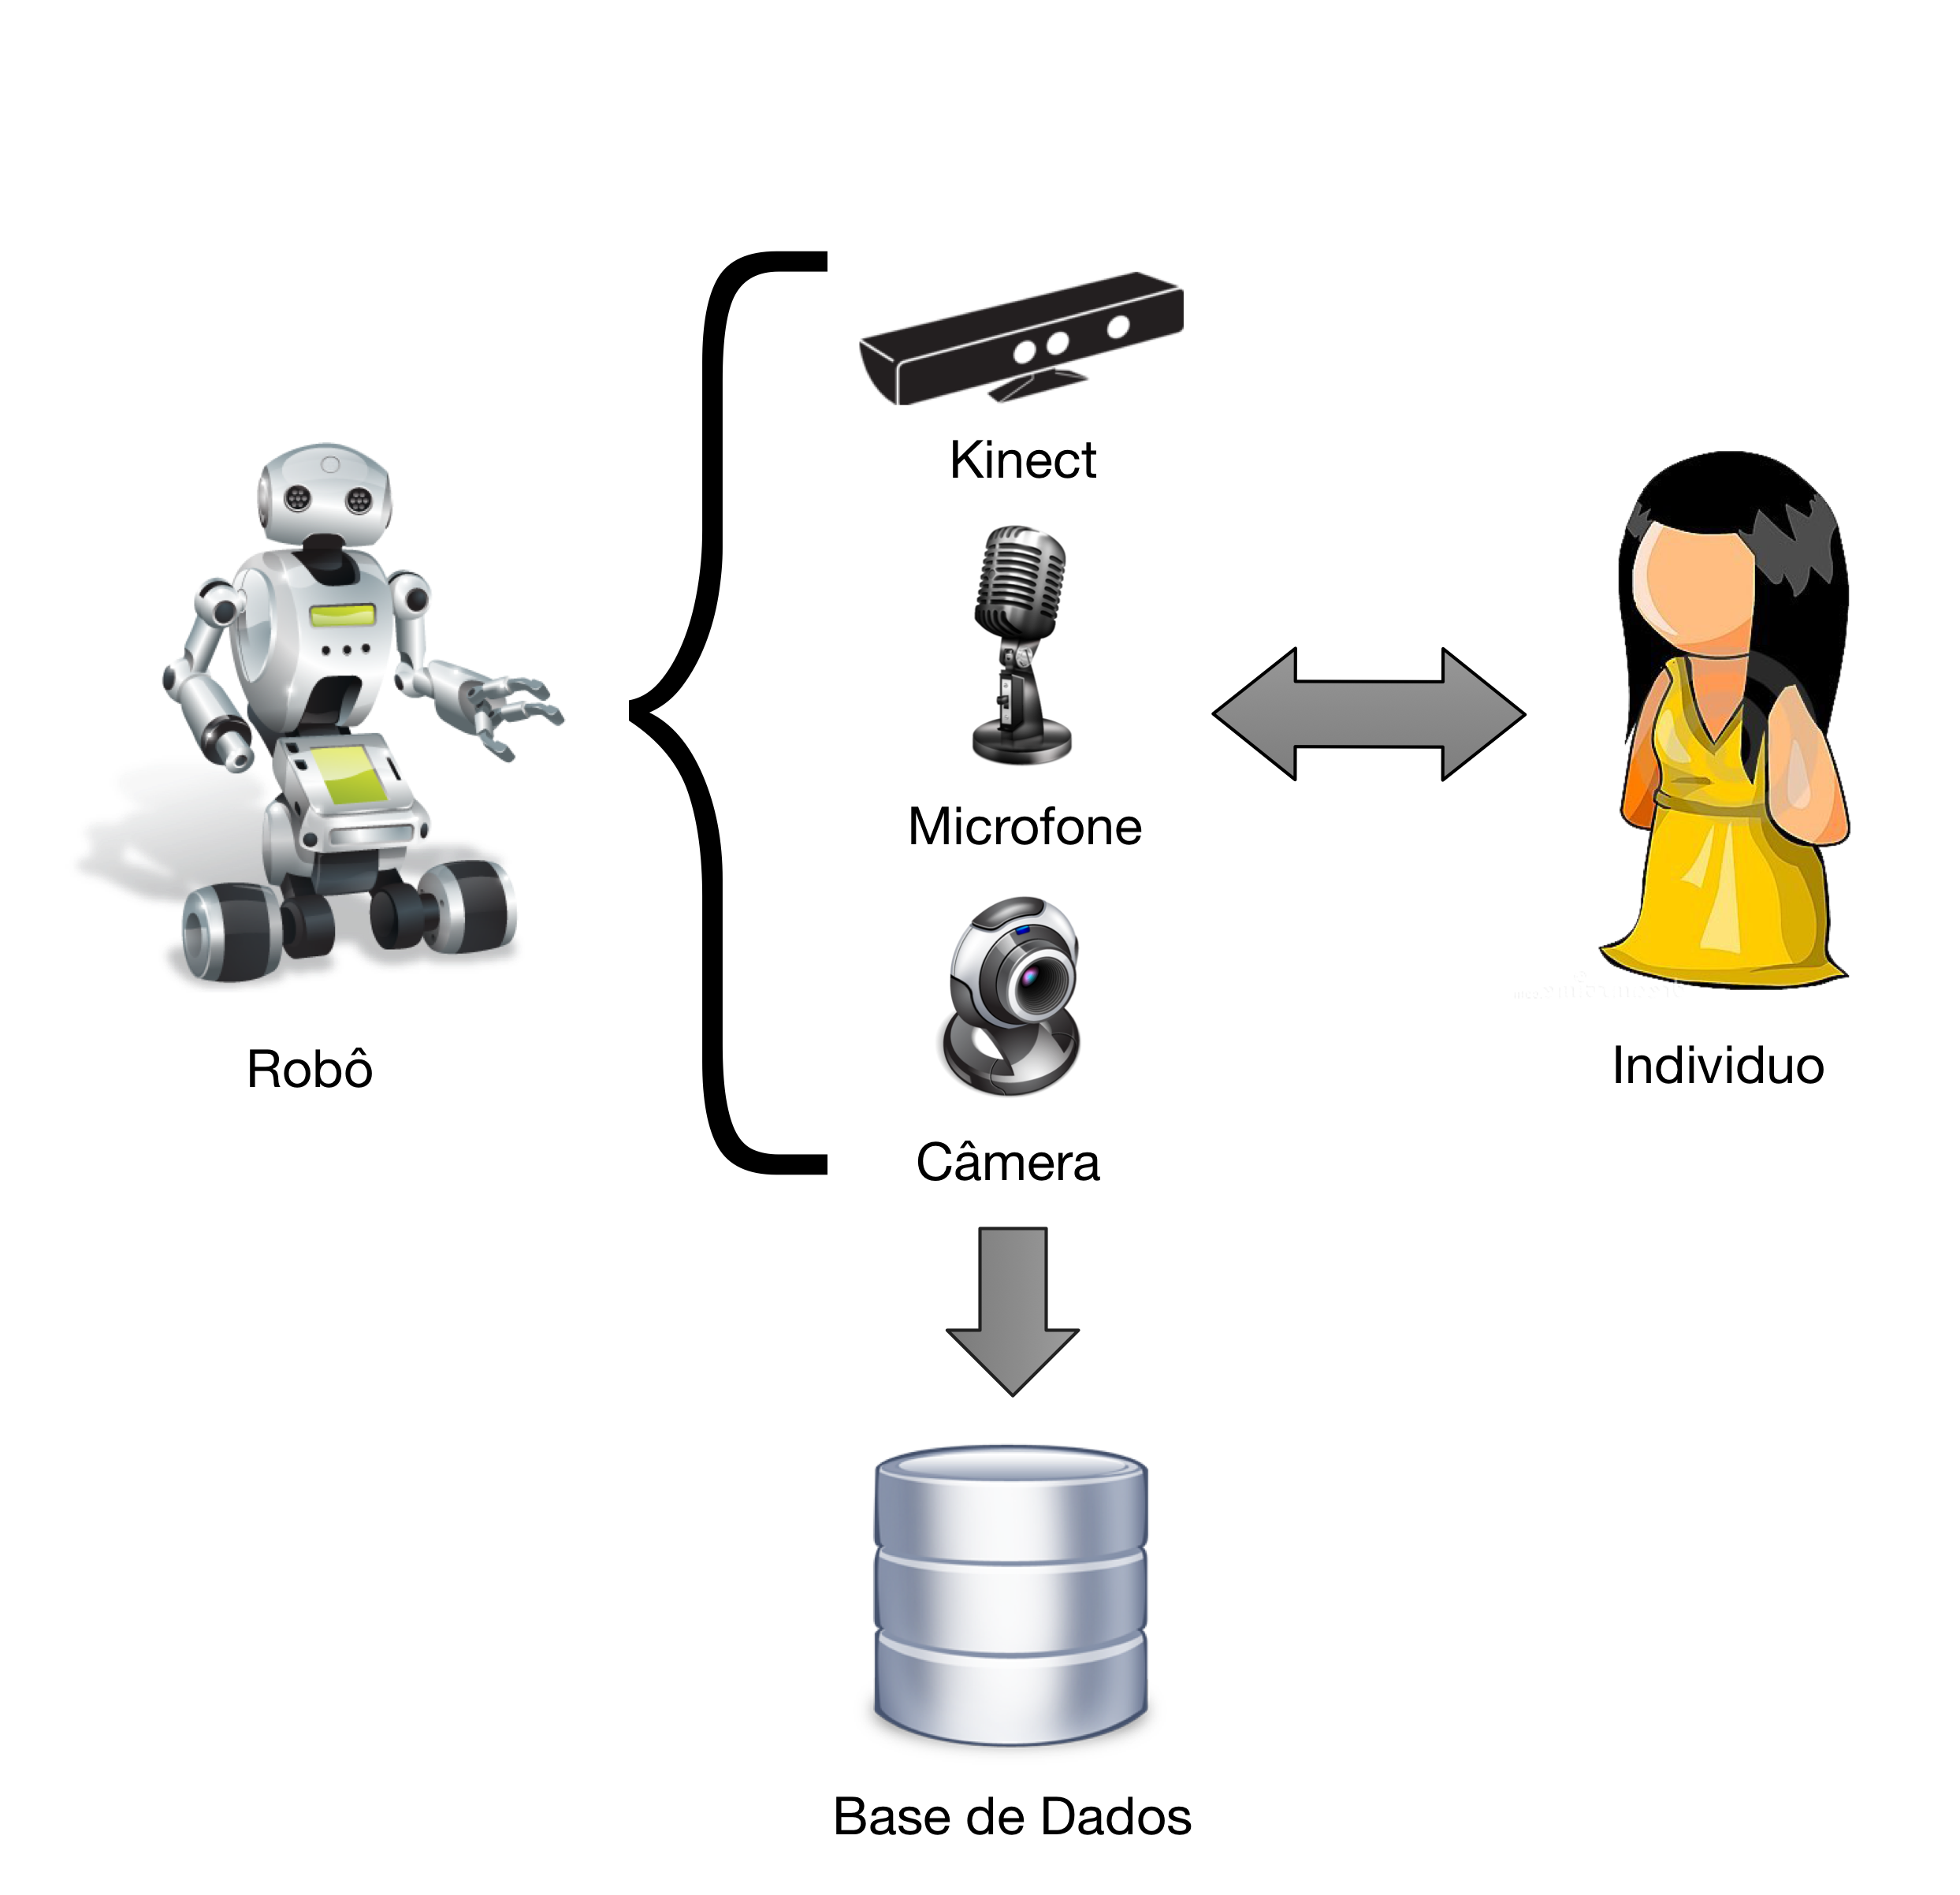
\includegraphics[scale=0.6]{images/captura_carac_individuo.png}
	\caption{Processo para a extração das características do individuo.}
	\label{fig:capturacaracteristicas}
\end{figure}

No processo apresentado pela figura \ref{fig:capturacaracteristicas}, o robô utiliza os sensores para identificar que o individuo iniciará uma interação com ele. Ao estabelecer o processo de interação, o robô utiliza um componente de \emph{log} que armazena todos os valores das variáveis que são utilizadas para determinar o perfil comportamental do individuo em um banco de dados. As variáveis são apresentadas em detalhes nas seções \ref{sec:variaveisindividuo} e \ref{sec:variaveisrobo}. Com as informações armazenadas determina-se através de um algoritmo de agrupamento, grupos que possuem perfis comportamentais similares, coletados e armazenados no banco de dados. Deve-se lembrar que as informações sobre o comportamento do individuo são direcionadas por um cenário de interação, como discutido por \citeonline{Jung:1991} em seu trabalho. 

Dessa forma, as variáveis aplicadas ao comportamento tem dependência do cenário de interação, porém as informações das variáveis etnográficas como idade, experiência computacional, sexo, local de origem, etnia, entre outras, são independentes do cenário. Existem alguns algoritmos na área de visão computacional que são capazes de identificar algumas variáveis etnográficas de maneira automática \cite{Yang:2007, Shan:2012, Ylioinas:2012, Samadi:2013, Amaral:2014}, porém para o trabalho desta tese, a coleta dessas informações será realizada através de um questionário pré interação já que esses algoritmos não fazem parte do objetivo principal do trabalho. As informações obtidas através do questionário serão inseridas no banco de dados complementando as informações de comportamento, que são separadas obtidas através da interação entre o ser humano e o robô através dos cenários de interação.

Na seção \ref{sec:variaveisindividuo} são detalhados os conjuntos de variáveis etnográficas e comportamentais com uma breve explicação dos objetivos esperados de cada uma das variáveis coletadas. A seção \ref{sec:variaveisrobo} detalha as variáveis que serão consideradas para o perfil do robô, apresentando também uma explicação sobre os objetivos de cada uma das variáveis.

\subsection{Selecionando as Variáveis para o Individuo}
\label{sec:variaveisindividuo}

Essa seção apresenta os conjuntos de variáveis que são consideradas nesse trabalho como a base de informações para seu desenvolvimento. Dois conjuntos são apresentados, o conjunto de variáveis etnográficas, seguido pelo conjunto de variáveis comportamentais que é o principal foco deste trabalho.

\subsubsection{Conjunto de Variáveis Etnográficas}
\label{sec:variaveisetnograficas}

O objetivo das variáveis etnográficas é identificar qual a experiência social e computacional de cada indivíduo. Além da experiência, também pode-se obter informações sobre a idade, gênero, local de nascimento ou origem do indivíduo. Todas essas informações são relevantes para verificar a existência de uma possível relação entre as variáveis etnográficas e comportamentais. A lista apresentada a seguir define as variáveis etnográficas e uma breve explicação sobre o significado de cada uma das variáveis.

\begin{enumerate}
	\item \textbf{Idade}: informa a idade do indivíduo.
	\item \textbf{Gênero}: informa o sexo biológico do indivíduo.
	\item \textbf{Local de Nascimento}: informa qual o local de nascimento do indivíduo. Essa variável auxiliará a determinar a base cultural do indivíduo.
	\item \textbf{Etnia}: informa a origem da família do indivíduo. Outra variável que auxilia na determinação da base cultural do indivíduo.
	\item \textbf{Quantidade de \emph{Gadgets}}: informa a quantidade de \emph{gadgets} que o indivíduo possui, ajudando a identificar qual a experiência e o contato dele com a tecnologia.
	\item \textbf{Contato prévio com Robôs}: informa apenas se o indivíduo já possuiu algum contato com robôs. Auxiliará a determinar o contato com a tecnologia, principalmente com robôs que poderá influenciar no seu comportamento durante a interação.
	\item \textbf{Tipos de Robôs}: informa quais são os tipos de robôs que o indivíduo teve contato. Os tipos poderão ser robôs \emph{Pet}, Humanoides, Androides, Móveis, entre outros. Essa variável é um complemento da variável ``Contato prévio com Robôs''.
	\item \textbf{Quantidade de cidades visitadas}: informa a quantidade de cidades que o indivíduo já visitou além da sua cidade natal. É importante para identificar o contato com outros tipos de cultura. Isso poderá influenciar no comportamento definido por sua cultura.
	\item \textbf{Quantidade de cidades que morou}: informa a quantidade de cidades que o indivíduo já morou além da sua cidade natal. É importante para identificar a vivência com outros tipos de cultura. Isso poderá influenciar no comportamento definido por sua cultura.
	\item \textbf{Quantidade de países visitadas}: informa a quantidade de países que o indivíduo já visitou além da sua cidade natal. É importante para identificar o contato com outros tipos de cultura. Isso poderá influenciar no comportamento definido por sua cultura.
	\item \textbf{Quantidade de países que morou}: informa a quantidade de países que o indivíduo já morou além da sua cidade natal. É importante para identificar a vivência com outros tipos de cultura. Isso poderá influenciar no comportamento definido por sua cultura.
\end{enumerate}

Em diversos trabalhos da seção \ref{sec:proxemicsihr}, onde a questão cultural do indivíduo é abordada, são discutidos que influência dela sobre o comportamenteo do o indivíduo. Contudo, a cultura é tratada como a origem do indivíduo, por exemplo, no trabalho de \citeonline{Eresha:2013}. Entretanto, a questão cultural na vida de uma pessoa é mais abrangente, está relacionada a experiência adquirida ao longo de sua vivência social. Dessa forma, o conjunto de variáveis apresentado acima tem como objetivo mapear de forma abstrata a experiência social do indivíduo, com o intuito de tornar o comportamento menos dependente da origem e talvez de sua experiência prévia.

Nesse trabalho, as informações levantadas nessa seção serão adquiridas através de questionários pré testes de interação. Em trabalhos futuros serão feitos estudos para identificar essas informações de maneira interativa através do próprio robô.

\subsubsection{Conjunto de Variáveis Comportamentais}
\label{sec:variaveiscomportamentais}

Variáveis comportamentais tem como principal objetivo identificar o comportamento do indivíduo. Nesse trabalho o comportamento está diretamente relacionado com cenários de interação social. As variáveis comportamentais são coletadas a partir de informações sobre as posições corporais e expressões faciais do indivíduo, tornando possível uma análise com base em teorias de linguagem corporal. As análises realizadas a partir da linguagem corporal, tem por base o trabalho apresentado por \citeonline{Lambert:2008}. O conjunto de variáveis comportamentais apresentados nessa seção não são utilizadas apenas para extrair o perfil do indivíduo, mas também para avaliar se a ação realizada pelo robô gerou uma reação positiva ou negativa no indivíduo. A lista apresentada a seguir define as variáveis comportamentais e uma breve explicação sobre o objetivo de cada uma das variáveis.

\begin{enumerate}
	\item \textbf{Expressões Faciais}: é possível identificar se a reação do indivíduo foi positiva ou negativa, a partir de uma ação do robô. Existem seis expressões bases que combinadas formam diversas outras~\cite{Bihan:2014}. Contudo, nesse trabalho será considerado apenas as seis expressões bases classificadas em dois grupos: expressões faciais positivas e expressões faciais negativas. O intuito dessa variável é realizar a avaliação da ação do robô com base nas expressões faciais do indivíduo.
	\item \textbf{Tempo de Transição entre as Zonas Sociais}: identificar o tempo que o indivíduo ficou confortável com a presença do robô a medida que esse diminuiu a distância entre eles.
	\item \textbf{Frequência do Olhar em direção ao Robô}: identificar se o indivíduo mantém o olhar ao robô, sendo possível saber se a interação está continua ou não. Isso pode influenciar se o robô está interagindo de maneira confortável ao indivíduo ou se esse está incomodado com a presença do robô.
	\item \textbf{Tempo do Olhar}: é possível mensurar o interesse do indivíduo durante a interação através do tempo que ele permanece com o olhar fixo no robô. Quanto maior o tempo do olhar, maior o interesse na interação do indivíduo.
	\item \textbf{Orientação dos ombros}: Auxilia a mensurar o interesse do indivíduo durante a interação, analisando se os ombros possuem a mesma orientação que a cabeça e também uma orientação em direção ao indivíduo que interage com o robô. Além disso, é possível determinar através do alinhamento do quadril com o ombro do indivíduo o ângulo de inclinação de seu torso. A inclinação do torso auxilia a identificar o interesse do indivíduo na interação, para isso basta verificar se ele está inclinado em direção ao robô para determinar um interesse positivo.
	\item \textbf{Orientação do quadril}: Auxilia a mensurar o interesse do indivíduo durante a interação. A orientação do quadril em direção ao robô ou na direção oposta auxilia a determinar o grau de interesse do indivíduo na interação. Quando mais alinhado à direção do robô, maior o interesse do indivíduo na interação.
	\item \textbf{Estilo da Voz}: é importante, pois pode determinar a reação que o indivíduo terá após a interação via áudio com o robô. Além disso, é possível determinar se o indivíduo está confortável ou não durante a interação, analisando o tom de sua voz ao responder o robô. Nesse trabalho, será considerado somente o canal de resposta ao indivíduo. A análise do tom da voz do indivíduo não será considerado nesta tese e ficará para trabalhos futuros de aprimoramento do componente de análise comportamental em IHR.
\end{enumerate}

\subsection{Selecionando as Variáveis para o Robô}
\label{sec:variaveisrobo}
Além das variáveis referentes ao perfil do indivíduo, deve-se considerar também as informações sobre o robô uma vez que sua aparência pode influenciar na reação das pessoas durante a interação~\cite{Hegel:2009}. Coletar as variáveis do robô pode auxiliar a identificar quais são os principais fatores que tornam a interação humano-robô desconfortável ou com menos qualidade. Dessa forma, foi definido um conjunto de variáveis que pudessem caracterizar da melhor maneira fatores do robô, referente a sua aparência, que influenciam na IHR. Esse conjunto de variáveis é apresentado a seguir:

\begin{enumerate}
	\item \textbf{Altura}: A altura do robô para identificar a influência da diferença entre alturas de robôs e humanos.
	\item \textbf{Volume}: O volume ocupado pelo robô pode influenciar no conforto da interação, uma vez que quando o robô atingir uma zona social mais próxima do indivíduo pode causar uma sensação claustrofóbica a ele.
	\item \textbf{Tipo do Robô}: Segundo \citeonline{Choi:2014}, robôs possuem dois tipos: Autônomos e Tele-operados. Essa variável define o quanto de intervenção humana é necessário para que o robô possa executar a tarefa objetivo.
	\item \textbf{Classificação do Robô}: Segundo \citeonline{Dobra:2014} classificar um robô é uma tarefa muito complexa e pode envolver diversas variáveis. Dessa forma, para essa tese será considerado uma classificação mais simples. O robô deve ser classificado como: fixo, móvel com rodas, móvel bípede, móvel quadrupede, móvel com manipuladores. Outras classificações podem ser inseridas conforme a necessidade e inclusão de novos robôs.
	\item \textbf{Aparência Física}: Essa variável descreve se o robô possui uma aparência amigável ou agressiva.
	\item \textbf{Nível de Ruído}: Determina qual o nível de ruído que os atuadores do robô podem gerar de tal forma, que possa influenciar na interação humano-robô.
\end{enumerate}

Além das variáveis que definem as características, é necessário também o mapeamento das ações que o robô irá executar para que exista uma avaliação dessa após a reação do indivíduo. As variáveis que compõem as informações do perfil comportamental do robô são:

\begin{enumerate}
	\item \textbf{Aproximação}: Forma de aproximação do robô ao indivíduo. Pode ser classificada entre rápida, devagar, brusca ou suave.
	\item \textbf{Movimentação do Manipulador}: Caso exista um manipulador deve descrever como é feita a movimentação do manipulador em direção ao usuário. A classificação consiste em brusca ou suave.
	\item \textbf{Estilo de Voz}: Ao emitir algum tipo de som o robô deverá manter um estilo de voz para que seja possível simbolizar qual o tipo de mensagem ele deseja falar. A classificação será feita de maneira simplificada, considerando apenas se é um estilo educado ou agressivo.
	\item \textbf{Expressão Facial}: Ao iniciar o contato visual com o indivíduo, pode ocorrer diversas expressões do robô na tentativa de manter o conforto do indivíduo durante o processo de interação. Simplificando as expressões, de maneira similar ao apresentado na seção~\ref{sec:variaveiscomportamentais}, são consideradas apenas dois tipos de expressões realizadas pelo robô: amistoso e não-amistoso. As expressões faciais do robô serão executadas através do \emph{tablet} acoplado nele, conforme descrito na seção~\ref{sec:robo}.
\end{enumerate}

As variáveis comportamentais do robô definidas com o objetivo de executar uma tarefa de abordagem para estabelecer uma interação. Caso seja necessário adicionar novas variáveis a esse conjunto não haverá problema ao método apresentado ao longo da seção.

\section{Raciocinando com Base nas Interações Extraídas}
\label{sec:raciociniointeracao}

Com as variáveis comportamentais e etnográficas do indivíduo e do robô definidas é necessário definir o método que fará com que o robô seja capaz de aprender a interagir com seres humanos a partir das suas experiências passadas. No capitulo \ref{cap:rbc} foi apresentado a técnica de Raciocínio Baseado em Casos (RBC) que tem como principal objetivo o desenvolvimento de um sistema de conhecimento com base em experiências ou casos ocorridos anteriormente. RBC tem uma estrutura baseada em 4(quatro) pilares, são eles~\cite{Lopez:2013}: Resgatar, Reutilizar, Revisar e Reter. A figura~\ref{fig:rbc} apresenta a metodologia dessa tese, que engloba as quatro etapas do RBC.

\begin{figure}[ht!]
	\centering
	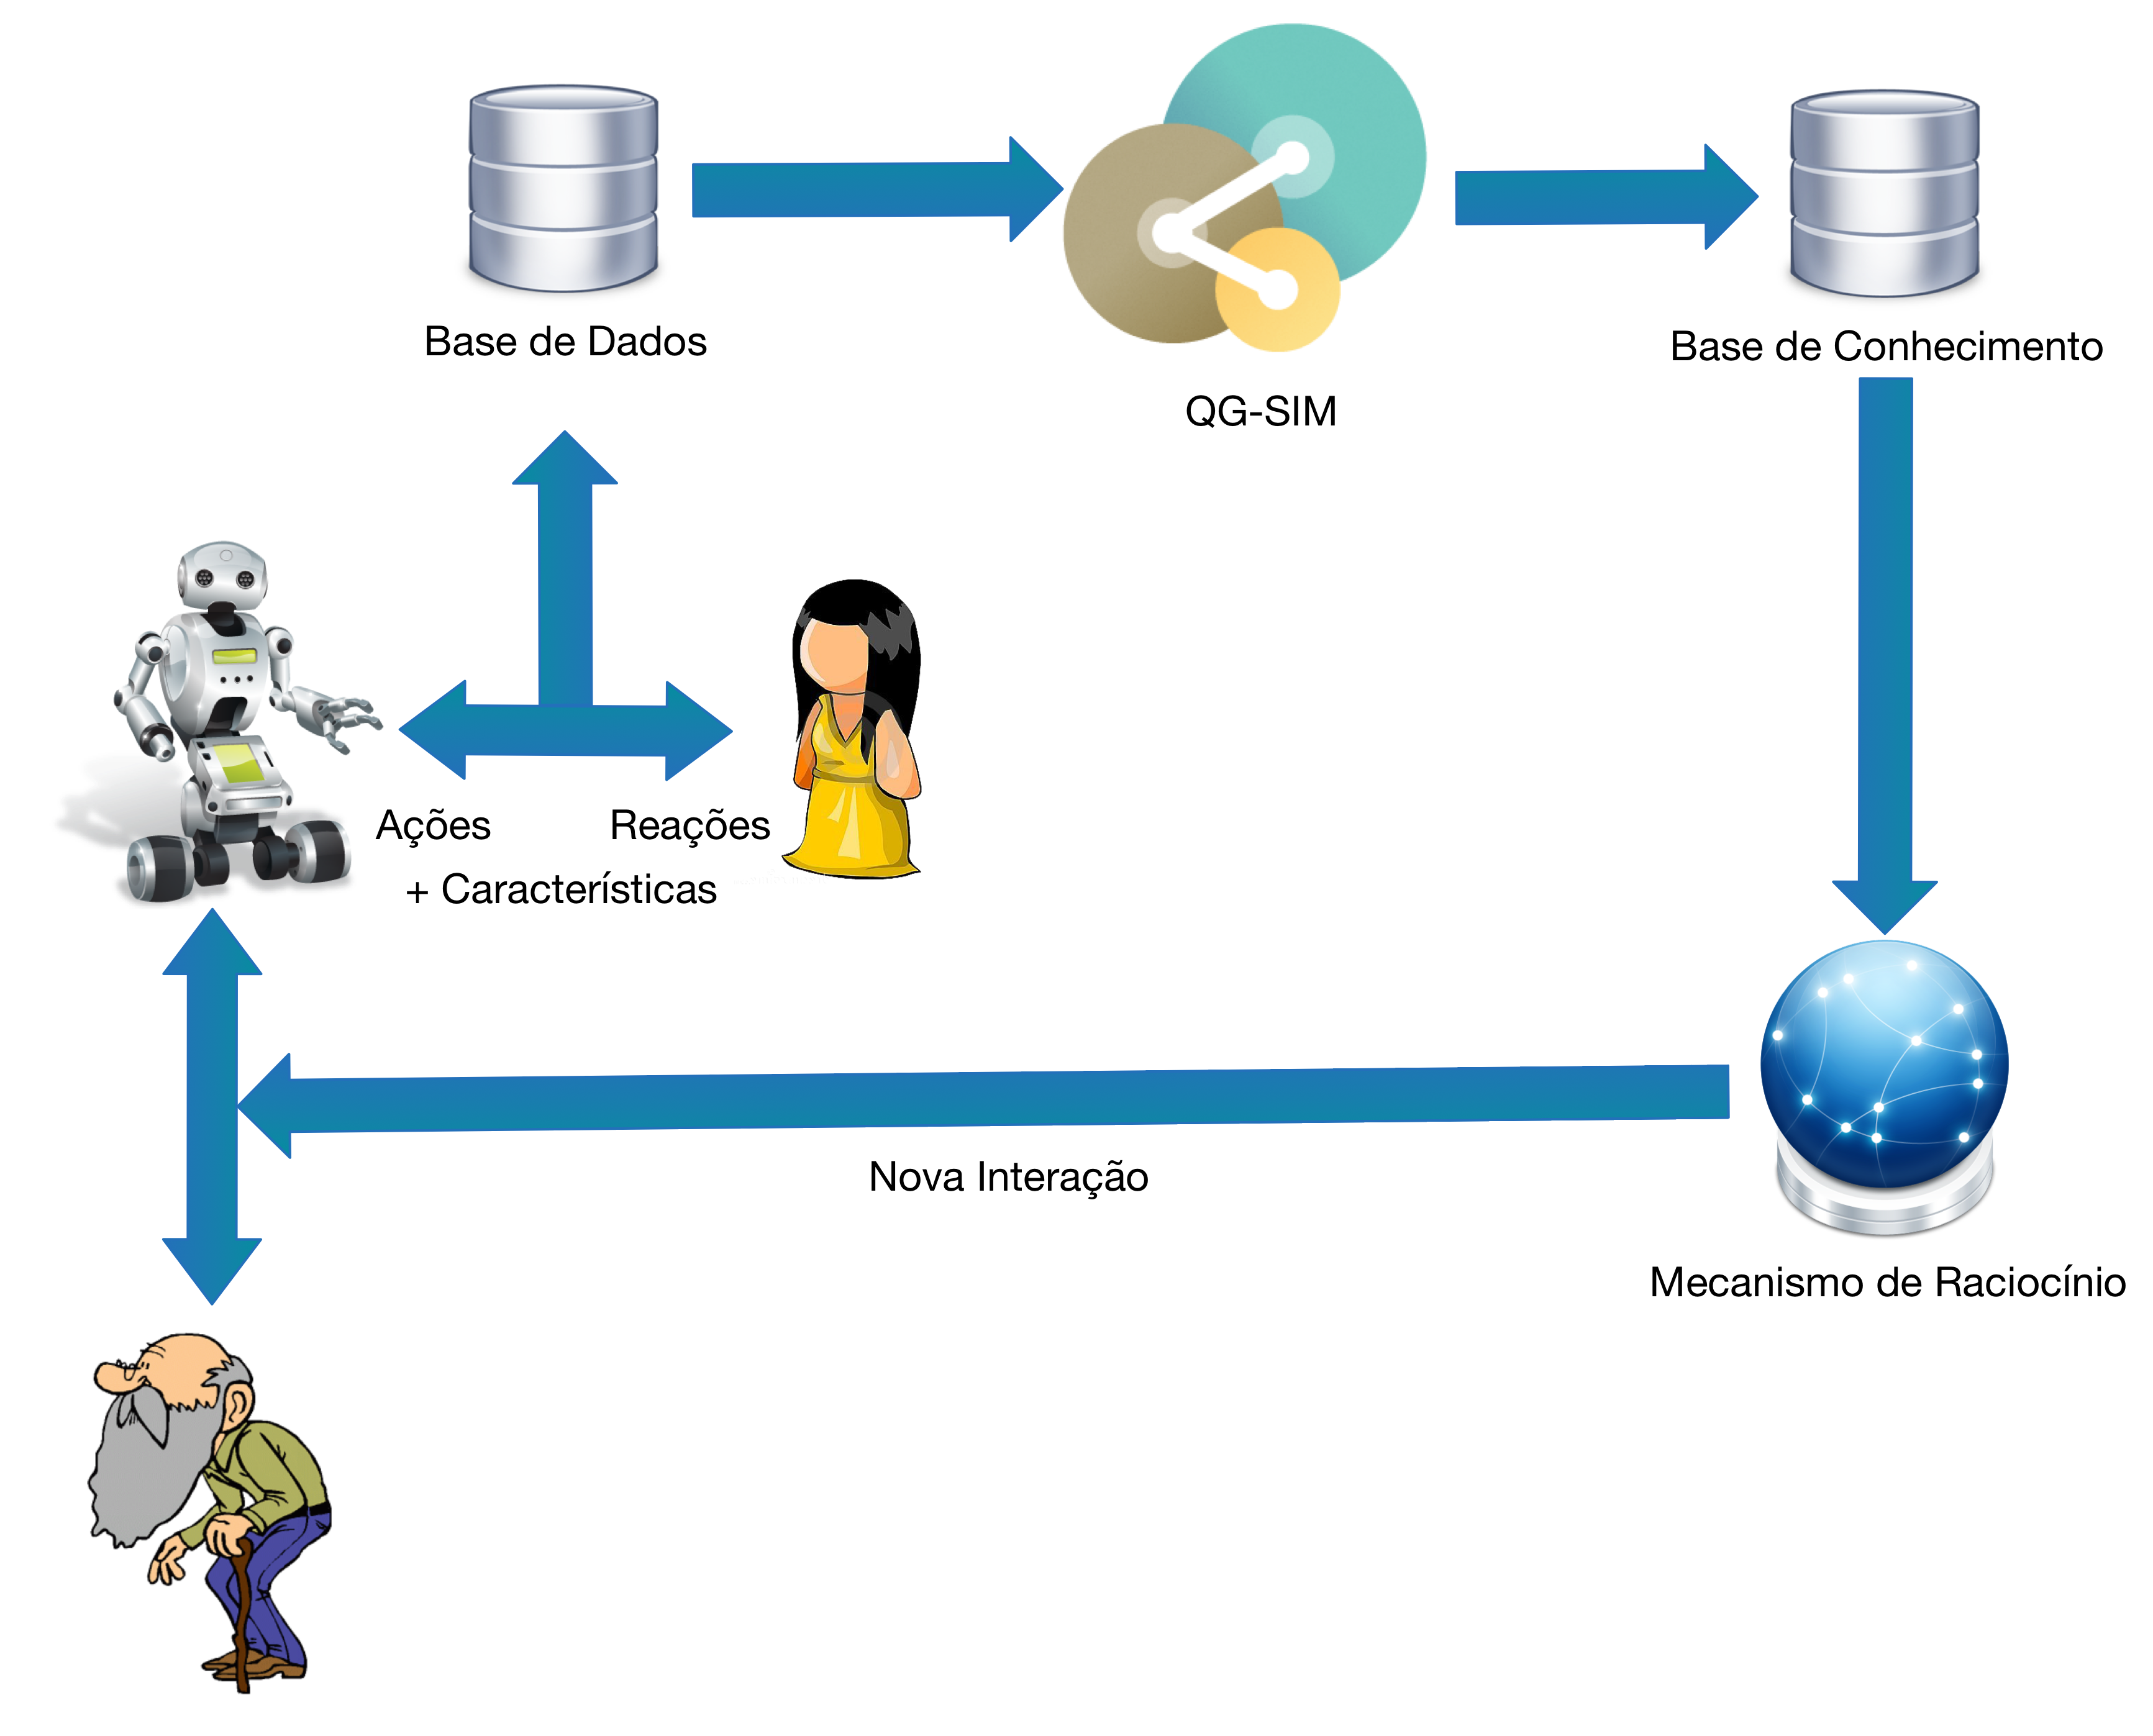
\includegraphics[width=\textwidth]{images/rbc_geral.png}
	\caption{Processo de Interação com Aprendizado baseado em Experiências Passadas.}
	\label{fig:rbc}
\end{figure}

A metodologia da figura~\ref{fig:rbc} tem início na interação entre o robô e a jovem localizada a sua frente. Durante a interação entre os dois o sistema coleta todas as reações da jovem para cada ação tomada pelo robô, de acordo com as variáveis descritas na seção~\ref{sec:extracaocaracteristicas}, que são armazenadas na base de dados. A base de dados formada a partir dessas informações é enviada ao algoritmo de agrupamento por similaridade QG-SIM (Quality Groups of Similarity, em inglês)~\cite{Masiero:2013}. Os grupos gerados pelo QG-SIM são analisados e inseridos na base de conhecimento formando os casos de pesquisa para novas interações. Quando ocorrer uma nova interação, como por exemplo o robô com o senhor na figura~\ref{fig:rbc}, o mecanismo de raciocínio realiza uma análise para que possa inferir qual o melhor caso a ser aplicado para interação entre o senhor e o robô. Mesmo que utilize casos existentes na base de conhecimento, todas as interações são armazenadas para manter o aprendizado sobre interações contínuo e sempre com o objetivo de manter o individuo confortável durante todo o processo. Na sequência serão detalhadas as fases do RBC de acordo com a metodologia apresentada na figura~\ref{fig:rbc}.

\subsection{Resgatar}
\label{sec:resgatar}

A partir de uma nova interação inicia-se o processo de resgate do caso que maximize as reações positivas de um determinado indivíduo a partir da ação que o robô realiza. Nessa fase a solução encontrada não poderá ser dada como exclusiva, pois quando trata-se de seres humanos a tarefa de determinar uma solução exata é complexa. Como para um mesmo perfil de indivíduo ou um perfil similar pode-se apresentar muitas soluções deve ser aplicado nessa fase um modelo probabilístico de tal forma, que a solução escolhida seja a que possui um maior valor de probabilidade no ponto de vista de maximizar a satisfação e o conforto do indivíduo.

Existem diversos métodos probabilísticos que podem ser aplicados nessa fase, como por exemplo, redes Bayesianas ou até mesmo conjunto de lógica nebulosa (Lógica \emph{Fuzzy}). Mesmo sendo o regaste de uma solução único para o caso, esse modelo possibilita que a solução selecionada para execução seja a melhor dentre todas as armazenadas dada uma distribuição probabilística. Selecionando o caso que será aplicado esse deve formar um conjunto de ações do robô para interação com o indivíduo, como é apresentado na próxima seção.

\subsection{Reutilizar}
\label{sec:reutilizar}

Após o resgate do caso que possui a maior similaridade de tornar a interação confortável ao indivíduo é necessário construir a sequência de ações que o robô irá executar. Para isso, deve-se considerar duas premissas. A primeira é que uma ação é dependente da anterior, pois caso essa premissa não seja considerada as ações que o robô executará não apresentarão nenhum sentido ao indivíduo. Isso faz com que esse modelo de reutilização seja considerado como temporal, onde uma ação futura depende de uma ação passada. A segundo premissa que deve ser considerada é que o indivíduo irá se comportar de maneira diferente da esperada em algum momento do processo de interação. Dessa maneira, deve-se realizar um novo resgate para a solução que maximiza o conforto da interação a partir daquele ponto onde a reação do indivíduo foi diferente do esperado.

\subsection{Reter}
\label{sec:reter}

Durante a interação entre o robô e um indivíduo as informações sobre o comportamento são armazenadas em um banco de dados. A partir desse banco de dados é realizado um agrupamento entre os perfis comportamentais que possuem uma certa similaridade. Para realizar esse agrupamento é utilizado um algoritmo chamado QG-SIM. O QG-SIM~\cite{Masiero:2013} mantém a qualidade da similaridade entre os perfis de um mesmo grupo, sendo dessa maneira, o algoritmo ideal para esse tipo de tarefa e cenário.

Com os grupos formados é utilizado uma processo definido por \citeonline{Masiero:2013} para gerar um perfil comum ao grupo. Esse perfil comum também pode ser considerado a centroide do grupo. O procedimento para encontrar a centroide do grupo auxilia a determinar o perfil que será inserido na base do conhecimento que é utilizada no processo de resgate e reutilização do sistema de RBC.

A opção de realizar esse processo de agrupamento para inserir um caso na base de conhecimento é importante, pois diminui a quantidade de casos para busca por parte do sistema de RBC. Diminuir o número de casos aumenta o desempenho do algoritmo fazendo com que o robô tenha uma resposta na interação mais rápida, evitando com que o indivíduo espere muito por uma ação do robô.

\subsection{Revisar}
\label{sec:revisar}

Com a base de conhecimento formada é executado um procedimento para verificar se existem perfis iguais ou similares a ponto que possam ser excluídos. Dessa maneira, é possível manter a base de conhecimento sempre com perfis exclusivos entre os existentes. Assim, é possível garantir que um número maior de indivíduos seja atendido pelo sistema de RBC.

Apesar da metodologia apresentada na figura~\ref{fig:rbc} possuir apenas um robô na interação, é possível transferir esse conhecimento a diversos robôs já que em sua arquitetura todo o sistema de RBC é extra robô. Assim, o processamento e conhecimento adquirido pelo sistema de RBC ficará disponível em um servidor ao qual todo robô que quiser utilizar dessas informações terá livre acesso.

Todo esse sistema será testado em um cenário de primeiro contato para interação entre dois agentes, nesse caso um robô e um indivíduo. O robô utilizado tem a locomoção feita através de rodas, porém sua altura é próxima da média dos seres humanos. As características do robô fazem com que ele seja apropriado para interações entre humanos e robôs.